\appendix
\section{Overview}
This document provides additional technical details, extra analysis experiments, more quantitative results and qualitative test results to the main paper.

In Sec.~\ref{sec:supp_pointnets} we provide more details on network architectures of PointNets and training parameters while Sec.~\ref{sec:supp_rgb_detector} explains more about our 2D detector. Sec.~\ref{sec:supp_bv} shows how our framework can be extended to bird's eye view (BV) proposals and how combining BV and RGB proposals can further improve detection performance. Then Sec.~\ref{sec:supp_more_exp} presents results from more analysis experiments. At last, Sec.~\ref{sec:supp_viz} shows more visualization results for 3D detection on SUN-RGBD dataset.
%We plan to release our training and testing code as well as our trained models for Frustum PointNets upon paper acceptance.

\section{Details on Frustum PointNets (Sec 4.2, 4.3)}
\label{sec:supp_pointnets}

\subsection{Network Architectures}
We adopt similar network architectures as in the original works of PointNet~\cite{qi2017pointnet} and PointNet++~\cite{qi2017pointnetplusplus} for our v1 and v2 models respectively. What is different is that we add an extra link for class one-hot vector such that instance segmentation and bounding box estimation can leverage semantics predicted from RGB images. The detailed network architectures are shown in Fig.~\ref{fig:arch}.

For v1 model our architecture involves point embedding layers (as shared MLP on each point independently), a max pooling layer and per-point classification multi-layer perceptron (MLP) based on aggregated information from global feature and each point as well as an one-hot class vector. Note that we do not use the transformer networks as in~\cite{qi2017pointnet} because frustum points are viewpoint based (not complete point cloud as in~\cite{qi2017pointnet}) and are already normalized by frustum rotation. In addition to XYZ , we also leverage LiDAR intensity as a fourth channel.

For v2 model we use set abstraction layers for hierarchical feature learning in point clouds. In addition, because LiDAR point cloud gets increasingly sparse as it gets farther, feature learning has to be robust to those density variations. Therefore we used a robust type of set abstraction layers -- multi-scale grouping (MSG) layers as introduced in~\cite{qi2017pointnetplusplus} for the segmentation network. With hierarchical features and learned robustness to varying densities, our v2 model shows superior performance than v1 model in both segmentation and box estimation.

\begin{figure*}
    \centering
    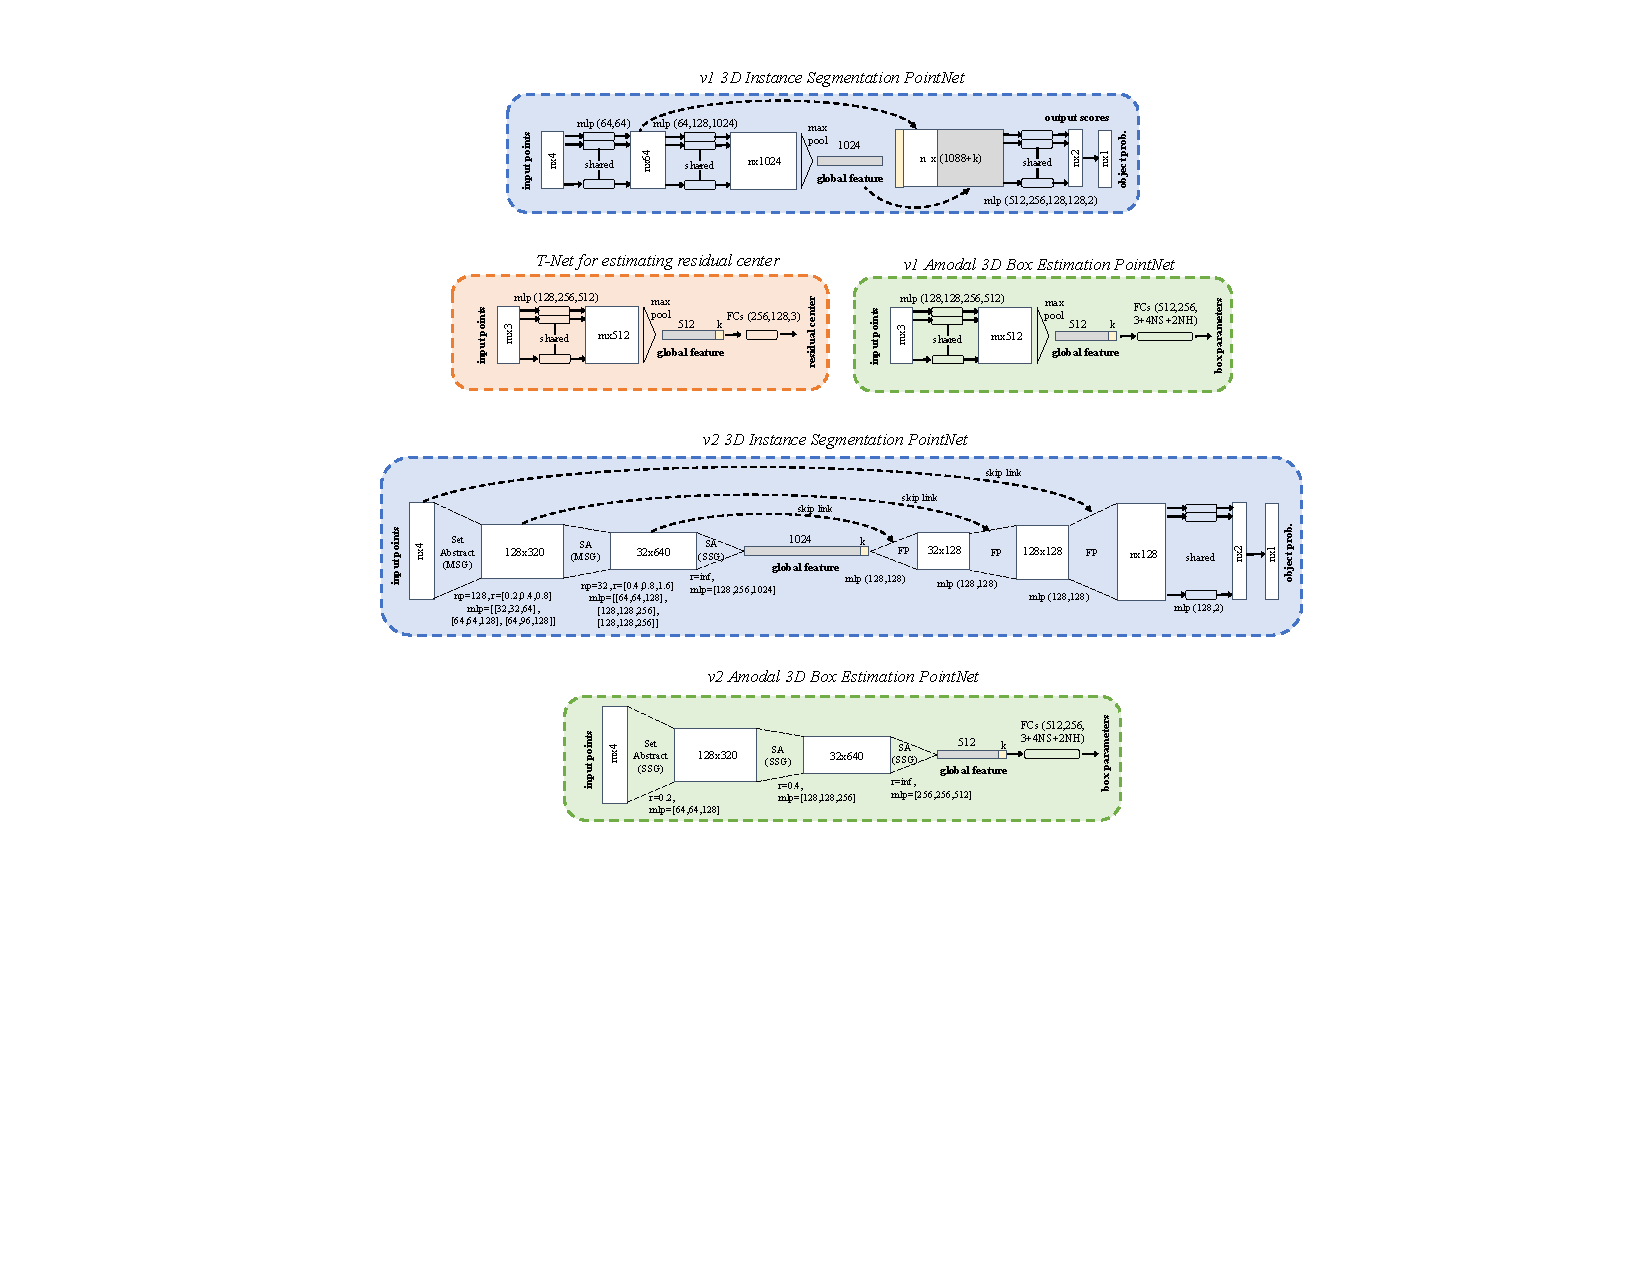
\includegraphics{./fig/arch}
    \caption{\textbf{Network architectures for Frustum PointNets.} v1 models are based on PointNet~\cite{qi2017pointnet}. v2 models are based on PointNet++~\cite{qi2017pointnetplusplus} set abstraction (SA) and feature propagation (FP) layers. The architecture for residual center estimation T-Net is shared for Ours (v1) and Ours (v2). The colors (blue for segmentaiton nets, red for T-Net and green for box estimation nets) of the network background indicate the coordinate system of the input point cloud. Segmentation nets operate in frustum coordinate, T-Net processes points in mask coordinate while box estimation nets take points in object coordinate. The small yellow square (or bar) concatenated with global features is class one-hot vector that tells the predicted category of the underlying object.}
    \label{fig:arch}
\end{figure*}

\subsection{Data Augmentation and Training}

\paragraph{Data augmentation} Data augmentation plays an important role in preventing model overfitting. Our augmentation involves two branches: one is 2D box augmentation and the other is frustum point cloud augmentation.

We use ground truth 2D boxes to generate frustum point clouds for Frustum PointNets training and augment the 2D boxes by random translation and scaling. Specifically, we firstly compute the 2D box height ($h$) and width ($w$) and translate the 2D box center by random distances sampled from Uniform[$-0.1w, 0.1w$] and Uniform[$-0.1h, 0.1h$] in u,v directions respectively. The height and width are also augmented by two random scaling factor sampled from Uniform[$0.9, 1.1$].

We augment each frustum point cloud by three ways. First, we randomly sample a subset of points from the frustum point cloud on the fly (1,024 for KITTI and 2,048 for SUN-RGBD). For object points segmented from our predicted 3D mask, we randomly sample 512 points from it (if there are less than 512 points we will randomly resample to make up for the number). Second, we randomly flip the frustum point cloud (after rotating the frustum to the center) along the YZ plane in camera coordinate (Z is forward, Y is pointing down). Thirdly, we perturb the points by shifting the entire frustum point cloud in Z-axis direction such that the depth of points is augmented. Together with all data augmentation, we modify the ground truth labels for 3D mask and headings correspondingly. 

\paragraph{KITTI Training} The object detection benchmark in KITTI provides synchronized RGB images and LiDAR point clouds with ground truth amodal 2D and 3D box annotations for vehicles, pedestrians and cyclists. The training set contains 7,481 frames and an undisclosed test set contains 7,581 frames. In our own experiments (except those for test sets), we follow ~\cite{chen2016monocular,cvpr17chen} to split the official training set to a train set of 3,717 frames and a val set of 3769 frames such that frames in train/val sets belong to different video clips. For models evaluated on the test set we train our model on our own train/val split where around 80\% of the training data is used such that the model can achieve better generalization by seeing more examples.

To get ground truth for 3D instance segmentation we simply consider all points that fall into the ground truth 3D bounding box as object points. Although there are sometimes false labels from ground points or points from other closeby objects (e.g. a person standing by), the auto-labeled segmentation ground truth is in general acceptable.

For both of our v1 and v2 models, we use Adam optimizer with starting learning rate 0.001, with step-wise decay (by half) in every 60k iterations. For all trainable layers except the last classification or regression ones, we use batch normalization with a start decay rate of 0.5 and gradually decay the decay rate to 0.99 (step-wise decay with rate 0.5 in every 20k iterations). We use batch size 32 for v1 models and batch size 24 for v2 models. All three PointNets are trained end-to-end.

Trained on a single GTX 1080 GPU, it takes around one day to train a v1 model (all three nets) for 200 epochs while it takes around three days for a v2 model. We picked the early stopped (200 epochs) snapshot models for evaluation.

\begin{table*}[t!]
\small
\centering
\begin{tabular}{l|ccc||ccc||ccc}
\hline
\multirow{2}{*}{Method} & \multicolumn{3}{c||}{Cars} & \multicolumn{3}{c||}{Pedestrians} & \multicolumn{3}{c}{Cyclists} \\ \cline{2-10} 
                        & Easy  & Moderate  & Hard  & Easy     & Moderate    & Hard    & Easy    & Moderate   & Hard   \\ \hline
SWC & \textbf{90.82} & 90.05 & 80.59 & 87.06 & \textbf{78.65} & 73.92 & \textbf{86.02} & \textbf{77.58} & \textbf{68.44} \\
RRC~\cite{Ren17CVPR} & 90.61 & \textbf{90.22} & \textbf{87.44} & 84.14 & 75.33 & 70.39 & 84.96 & 76.47 & 65.46 \\
Ours & 90.78 & 90.00 & 80.80 & \textbf{87.81} & 77.25 & \textbf{74.46} & 84.90 & 72.25 & 65.14 \\ \hline
\end{tabular}
\caption{\textbf{2D object detection} AP on KITTI \emph{test} set. Evaluation IoU threshold is 0.7. SWC is the first place winner on KITTI leader board for pedestrians and cyclists at the time of submission. Our 2D results are based on a CNN model on monocular RGB images.}
\label{tab:kitti_test_2d}
\end{table*}

\begin{table}[t!]
\centering
\begin{tabular}{l|ccc}
\hline
Subset & Easy    & Moderate    & Hard   \\ \hline
AP (2D) for cars   & 96.48 & 90.31 & 87.63 \\ \hline
\end{tabular}
\caption{\textbf{Our 2D object detection} AP on KITTI \emph{val} set.}
\label{tab:kitti_val_2d_detection}
\end{table}


\paragraph{SUN-RGBD Training} The data set consists of 10,355 RGB-D images captured from various depth sensors for indoor scenes (bedrooms, dining rooms etc.). We follow the same train/val splits as \cite{song2015sun,ren2016three} for experiments. The data augmentation and optimization parameters are the same as that in KITTI.

As to auto-labeling of instance segmentation mask, however, data quality is much lower than that in KITTI because of strong occlusions and tight arrangement of objects in indoor scenes (see Fig.~\ref{fig:sunrgbd_viz} for some examples). Nonetheless we still consider all points within the ground truth boxes as object points for our training. For 3D segmentation we get only a 82.7\% accuracy compared to around 90\% in KITTI. Due to the heavy noise in segmentation mask label, we choose to only train and evaluate on v1 models that has more strength in global feature learning than v2 ones. For future works, we think higher quality in 3D mask labels can greatly help the instance segmentation network training.


\section{Details on RGB Detector (Sec 4.1)}
\label{sec:supp_rgb_detector}

For 2D RGB image detector, we use the encoder-decoder structure (e.g. DSSD~\cite{fu2017dssd}, FPN~\cite{lin2016feature}) to generate region proposals from multiple feature maps using focal loss~\cite{lin2017focal} and use Fast R-CNN~\cite{girshick2015fast} to predict final 2D detection bounding boxes from the region proposals.

To make the detector faster, we take the reduced VGG~\cite{simonyan2014very} base network architecture from SSD~\cite{liu2016ssd}, sample half of the channels per layer and change all max pooling layers to convolution layers with $3\times3$ kernel size and stride of 2. Then we fine-tune it on ImageNet CLS-LOC dataset for 400k iterations with batch size of 260 on 10 GPUs. The resulting base network architecture has about 66.7\% top-1 classification accuracy on the CLS-LOC validation dataset and only needs about 1.2ms to process a $224\times224$ image on a NVIDIA GTX 1080.

We then add the feature pyramid layers~\cite{lin2016feature} from conv3\_3, conv4\_3, conv5\_3, and fc7, which are used to predict region proposals with scales of 16, 32, 64, 128 respectively. We also add an extra convolutional layer (conv8) which halves the fc7 feature map size, and use it to predict proposals with scale of 256. We use 5 different aspect ratios \{$\frac{1}{3}$, $\frac{1}{2}$, 1, 2, 3\} for all layers except that we ignore \{$\frac{1}{3}$, 3\} for conv3\_3. Following SSD, we also use normalization layer on conv3\_3, conv4\_3, and conv5\_3 and initialize the norm 40. For Fast R-CNN part, we extract features from conv3\_3, conv5\_3, and conv8 for each region proposal and concatenate all the features to predict class scores and further adjust the proposals. We train this detector from COCO dataset with $384\times384$ input image and have achieved 35.5 mAP on the COCO minival dataset, with only 10ms processing time for a $384\times384$ image on a single GPU.

Finally, we fine-tune the detector on car, people, and bicycle from COCO dataset, and have achieved 48.5, 44.1, and 40.1 for these three classes on COCO. We take this model and further fine-tune it on car, pedestrian, and cyclist from KITTI dataset. The final model takes about 30ms to process a $384\times1280$ image. To increase the recall of the detector, we also do detection from the center crop of the image besides the full image, and then merge the detections using non-maximum suppression.

Tab.~\ref{tab:kitti_test_2d} shows our detector's AP (2D) on KITTI test set. Our detector has achieved competitive or better results than current leading players on KITTI leader board. We've also reported our AP (2D) on val set in Tab.~\ref{tab:kitti_val_2d_detection} for reference.


% topdown view \todo{todo: do experiment}
% runtime (bn+conv combine...)
% v1 vs v2
% effects of training data amount \todo{todo: do experiment}
% effects of number of points? \todo{todo: do experiment. correlation between number of object points to 3D box accuracy}
% 2D AP results
% show coordinate systems (velo, rect, camera ...)

\section{Bird's Eye View PointNets (Sec 5.3)}
\label{sec:supp_bv}

In this section, we show that our 3D detection framework can also be extended to using bird's eye view proposals, which adds another orthogonal proposal source to achieve better overall 3D detection performance. We evaluate the results of car detection using LiDAR bird's eye view only proposals + point net (Ours(BV)), and combine frustum point net and bird's eye view point net using 3D non-maximum suppression (NMS) (Ours(Frustum + BV)). The results are shown in Table~\ref{tab:td_re}.

\paragraph{Bird's Eye View Proposal} Similar to MV3D~\cite{cvpr17chen} we use point features such as height, intensity and density, and train the bird's eye view 2D proposal net using the standard Faster-RCNN~\cite{ren2015faster} structure. The net outputs axis-aligned 2D bounding boxes in the bird's eye view. In detail, we discretize the projected point clouds into 2D grids with resolution of $0.1$ meter and with the depth and width range $0 ~ 60$ meters, which gives us the $600\times600$ input size. For each cell, we take the intensity and the density of the highest point and divide the heights into $7$ bins with the height of the highest point in each bin, which gives us $9$ channels in total. In Faster R-CNN, we use the VGG-16~\cite{simonyan2014very} with $3$ anchor scales ($16, 32, 48$) and $3$ aspect ratios ($\frac{1}{2}, 1, 2$). We train RPN and Fast R-CNN together using the approximate joint training.

To combine 3D detection boxes from frustum PointNets and the bird's eye view PointNets, we use 3D NMS with IoU threshold $0.8$. We also apply a weight (0.5) to 3D boxes from BV PointNets since it is a weaker detector compared with our frustum one.

\paragraph{Bird's Eye View (BV) PointNets} Similar to Frustum PointNets that take point cloud in frustum, segment point cloud and estimate amodal bounding box, we can apply PointNets to points in bird's eye view regions. Since bird's eye view is based on orthogonal projection, the 3D space specified by a BV 2D box is a 3D cuboid (cut by minimum and maximum height) instead of a frustum.

\paragraph{Results} Tab.~\ref{tab:td_re} (Ours BV) shows the APs we get by using bird's eye view proposals only (without and RGB information). We compare with two previous LiDAR only methods (VeloFCN~\cite{li2016vehicle} and MV3D (BV+FV)~\cite{cvpr17chen}) and show that our BV proposal based detector greatly outperforms VeloFCN on all cases and outperforms MV3D (BV+FV) on moderate and hard cases by a significant margin.

More importantly, we show in the last row of Tab.~\ref{tab:td_re} that bird's eye view and RGB view proposals can be combined to achieve an even better performance (\emph{3.8\%} AP improvement on hard cases).
Fig.~\ref{fig:frustum_vs_bv} gives an intuitive explanation of why bird's eye view proposals could help. In the sample frame shown: while our 2D detector misses some highly occluded cars (Fig.~\ref{fig:frustum_vs_bv}: left RGB image), bird's eye view based RPN successfully detects them (Fig.~\ref{fig:frustum_vs_bv}: blue arrows in right LiDAR image).


\begin{table}[h!]
    \centering
    \begin{tabular}{l|ccc}
    \hline
        Method & Easy & Moderate & Hard \\ \hline
        VeloFCN~\cite{li2016vehicle} & 15.20 & 13.66 & 15.98 \\
        MV3D~\cite{cvpr17chen} (BV+FV) & 71.19 & 56.60 & 55.30 \\ \hline
        Ours (BV) &  69.50 & 62.30 & 59.73 \\
        Ours (Frustum) & \textbf{83.76} & \textbf{70.92} & 63.65 \\
        Ours (Frustum + BV) & \textbf{83.76} & 70.91 & \textbf{67.47} \\ \hline
    \end{tabular}
    \caption{\textbf{3D object detection} AP on KITTI \emph{val} set. By using both proposals from RGB view (frustum) and bird's eye view (BV), we see a significant improvement in 3D AP (\emph{3.82\%}) on hard cases compared with our frustum only method. Ours (Frustum) here is the Ours (v2) in the main paper using PointNet++ architectures.}
    \label{tab:td_re}
\end{table}

\begin{figure}[h!]
    \centering
    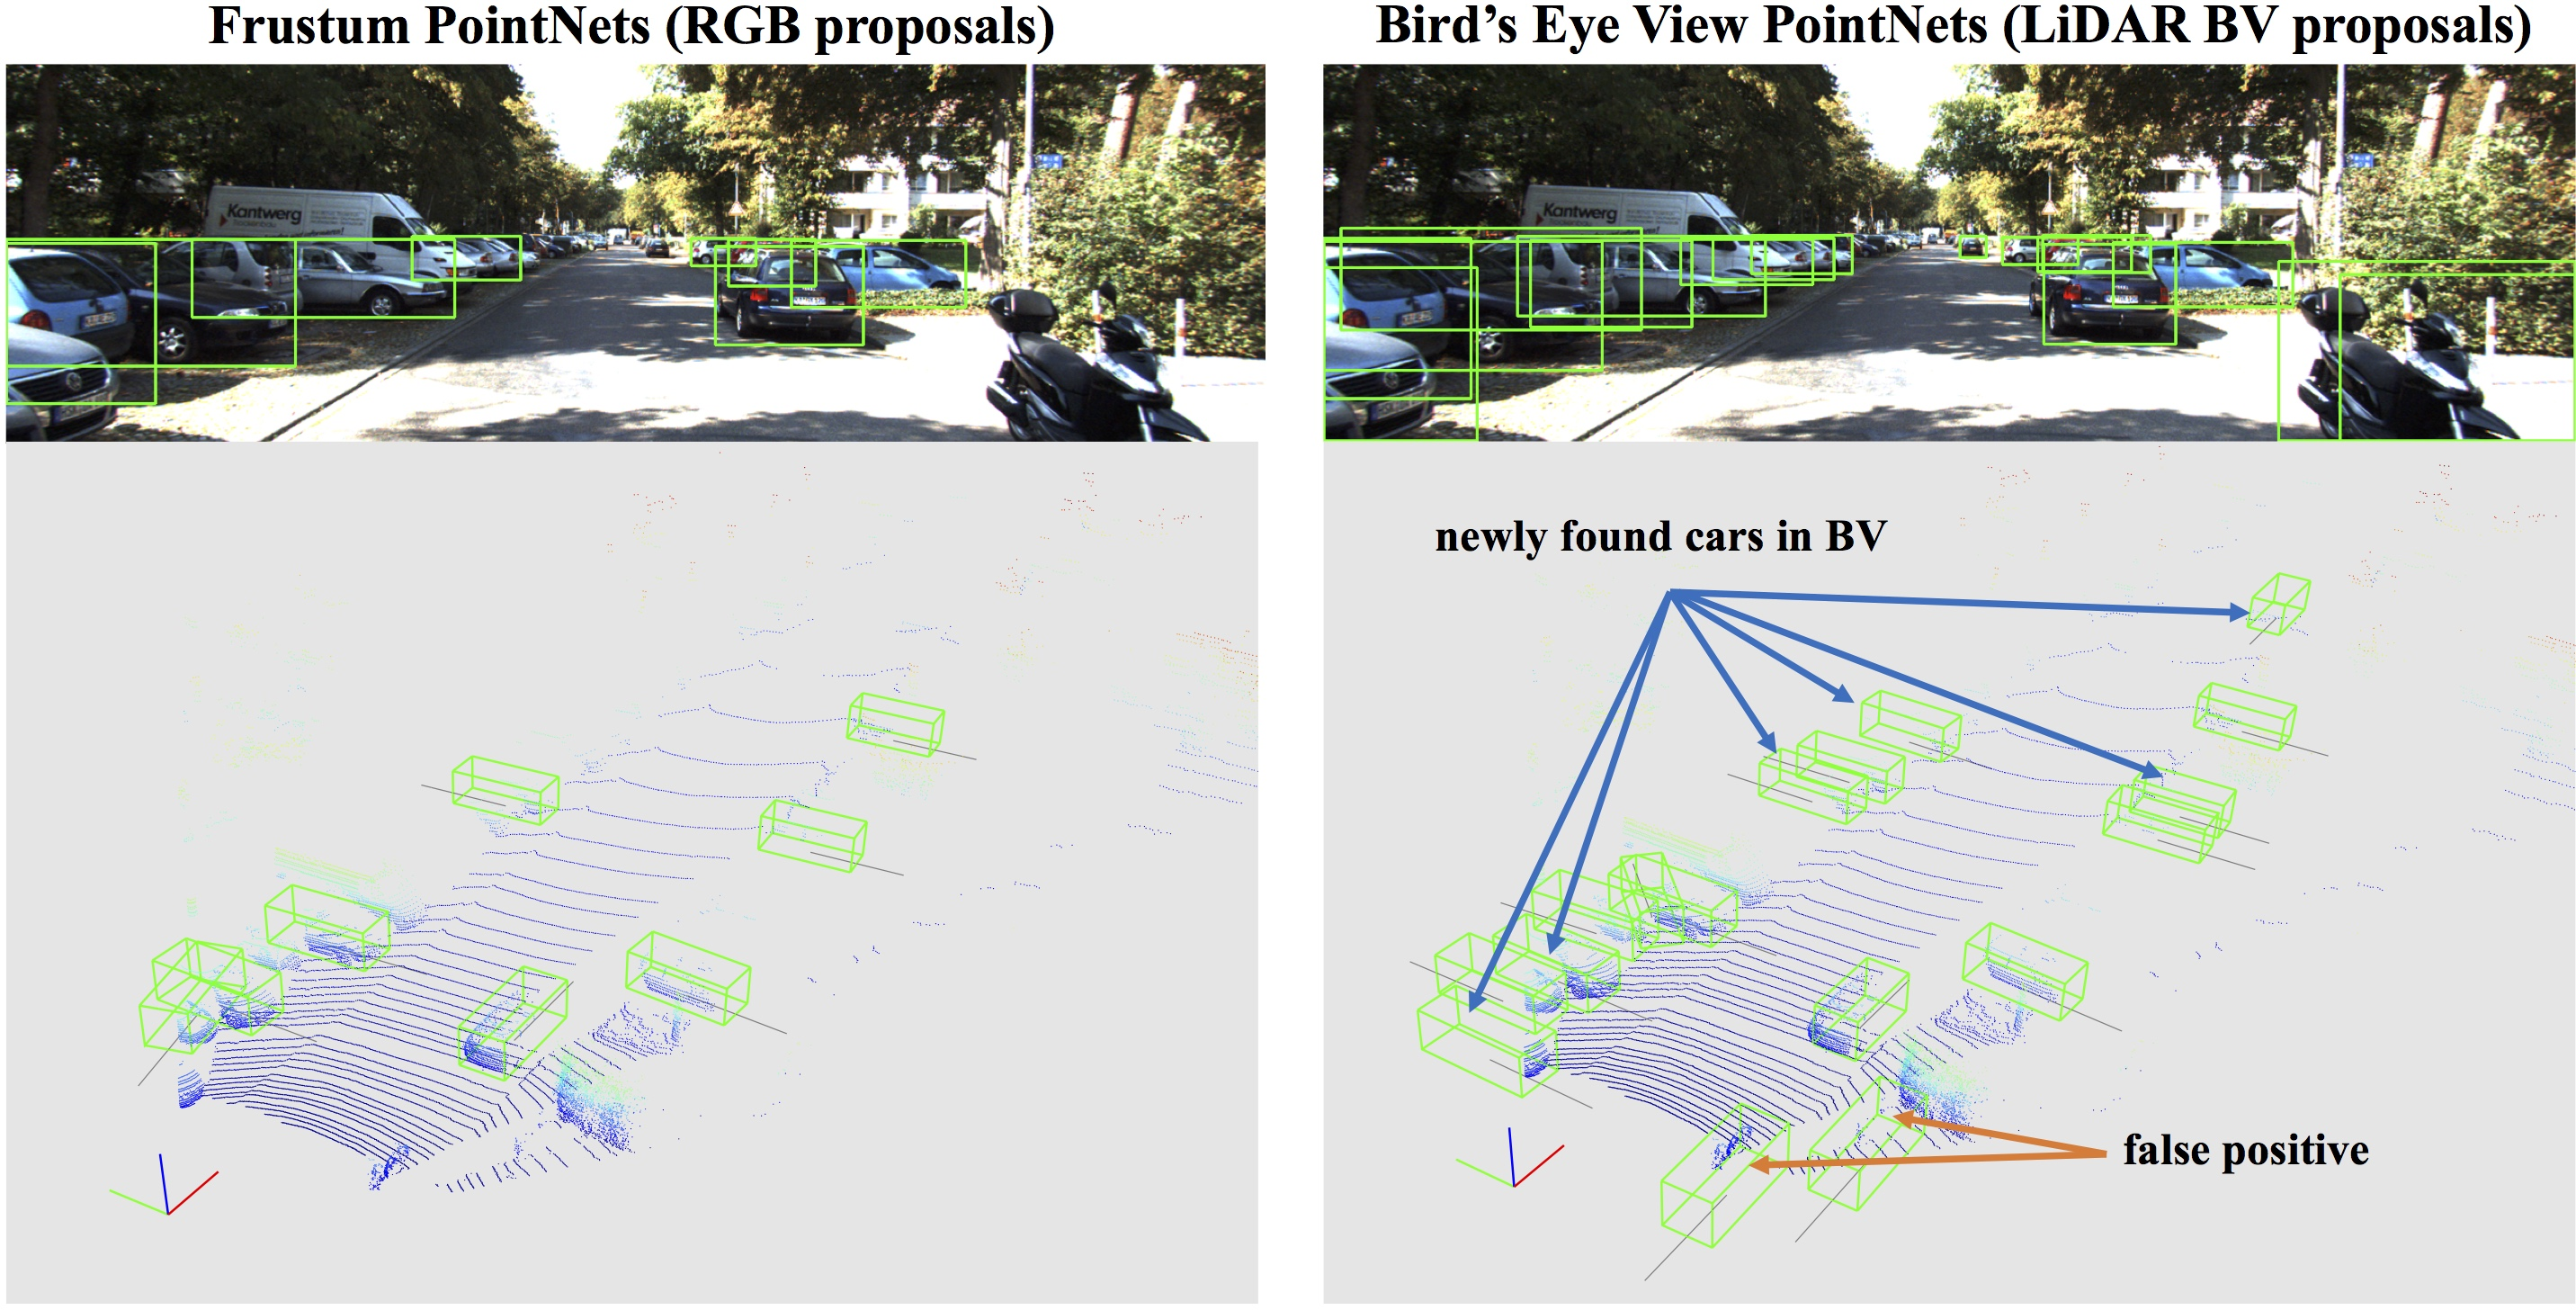
\includegraphics[width=\linewidth]{./fig/frustum_vs_bv.jpg}
    \caption{\textbf{Comparing Frustum PointNets and BV PointNets.} This is a scene with lots of parallel parking cars (sample 5595 from val set). \emph{Left} column shows 2D boxes from our 2D detector in image and 3D boxes from our Frustum PointNets in point cloud. \emph{Right} column shows 3D boxes from BV PointNets in point cloud and the 2D boxes (projected from the 3D detection boxes) in image. Note that 2D detection boxes from Ours (Frustum) that have box height less than 25 pixels or contain no LiDAR points in the frustum are not shown in the image.}
    \label{fig:frustum_vs_bv}
\end{figure}


\section{More Experiments (Sec 5.2)}
\label{sec:supp_more_exp}

\subsection{Effects of PointNet Architectures}
Table~\ref{tab:v1v2} compares PointNet~\cite{qi2017pointnet} (v1) and PointNet++~\cite{qi2017pointnetplusplus} (v2) architectures for instance segmentation and amodal box estimation. The v2 model outperforms v1 model on both tasks because 1) v2 model learns hierarchical features that are richer and more generalizable; 2) v2 model uses multi-scale feature learning that adapts to varying point densities. Note that the ours (v1) model corresponds to first row of Table~\ref{tab:v1v2} while the ours (v2) links to the last row.

\begin{table}[h!]
\centering
\begin{tabular}{cc|cc}
\hline
seg net & box net & seg acc. & box acc. \\ \hline
v1   & v1   & 90.6 & 74.3  \\
v2   & v1   & \textbf{91.0} & 74.7 \\
v1   & v2   & 90.6 & 76.0 \\
v2   & v2   & \textbf{91.0}  & \textbf{77.1} \\ \hline
\end{tabular}
\caption{\textbf{Effects of PointNet architectures.} Metric is 3D box estimation accuracy with IoU=0.7.}
\label{tab:v1v2}
\end{table}

\subsection{Effects of Training Data Size}

Recently \cite{sun2017revisiting} observed linear improvement in performance of deep learning models with exponential growth of data set size. In our Frustum PointNets we observe similar trend (Fig.~\ref{fig:training_data_size}). This trend indicates a promising performance potential of our methods with larger datasets.

We train three separate group of Frustum PointNets on three sets of training data and then evaluate the model on a fixed validation set (1929 samples). The three data points in Fig.~\ref{fig:training_data_size} represent training set sizes of 1388, 2776, 5552 samples (0.185x, 0.371x, 0.742x of the entire trainval set) respectively. We augment the training data such that the total amount of samples are the same for each of the three cases (20x, 10x and 5x augmentation respectively). The training set and validation set are chosen such that they don't share frames from the same video clips.

\begin{figure}[h!]
    \centering
    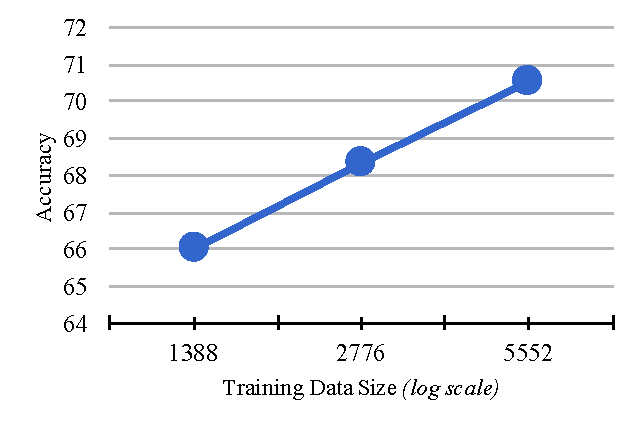
\includegraphics[width=0.6\linewidth]{./fig/training_data_amount.pdf}
    \caption{\textbf{Effects of training data size.} Evaluation metric is 3D box estimation accuracy (IoU threshold 0.7). We see a clear trend of linear improvement in accuracy with exponential growth of training data size.}
    \label{fig:training_data_size}
\end{figure}

\subsection{Runtime and Model Size}
\label{sec:runtime}
In Table~\ref{tab:runtime}, we show decomposed runtime cost (inference time) for our frustum PointNets (v1 and v2). The evaluation is based on TensorFlow~\cite{abadi2016tensorflow} with a NVIDIA GTX 1080 and a single CPU core. While for v1 model frustum proposal (with CNN and backprojection) takes the majority time, for v2 model since a PointNet++~\cite{qi2017pointnetplusplus} model with multi-scale grouping is used, computation bottleneck shifts to instance segmentation. Note that we merge batch normalization and FC/convolution layers for faster inference (since they are both linear operation with multiply and sum), which results in close to 50\% speedup for inference.

CNN model has size 28 MB. v1 PointNets have size 19MB. v2 PointNets have size 22MB. The total size is therefore 47MB for v1 model and 50MB for v2 model.

\begin{table}[h!]
\small
\centering
\begin{tabular}{c|ccc|c}
\hline
Model & Frustum Proposal & 3D Seg &  Box Est. & Total \\ \hline
v1 & 60 ms & 18 ms & 10 ms & 88 ms \\ 
v2 & 60 ms & 88 ms & 19 ms & 167 ms \\ \hline
\end{tabular}
\caption{\textbf{3D detector runtime.} Thirty-two region proposals used for frustum-based PointNets. 1,024 points are used for instance segmentation and 512 points are used for box estimation.}
\label{tab:runtime}
\end{table}

\section{Visualizations for SUN-RGBD (Sec 5.1)}
\label{sec:supp_viz}

In Fig.~\ref{fig:sunrgbd_viz} we visualize some representative detection results on SUN-RGBD data. We can see that compared with KITTI LiDAR data, depth images can be popped up to much more dense point clouds. However even with such dense point cloud, strong occlusions of indoor objects as well as the tight arrangement present new challenges for detection in indoor scenes.

In Fig.~\ref{fig:sunrgbd_ap} we report the 3D AP curves of our Frustum PointNets on SUN-RGBD val set. 2D detection APs of our RGB detector are also provided in Tab.~\ref{tab:kitti_val_2d_detection} for reference. 

% visualization on SUN-RGBD? \todo{todo: do visualization}
% visualization of instance segmentation (on OOS categories...)?  \todo{todo: do visualization}
% AP curves for our detector on KITTI
% AP curves for our detector on SUN-RGBD
% video for detection results (3 scenes) \todo{todo: do visualization}

\begin{figure*}[t!]
    \centering
    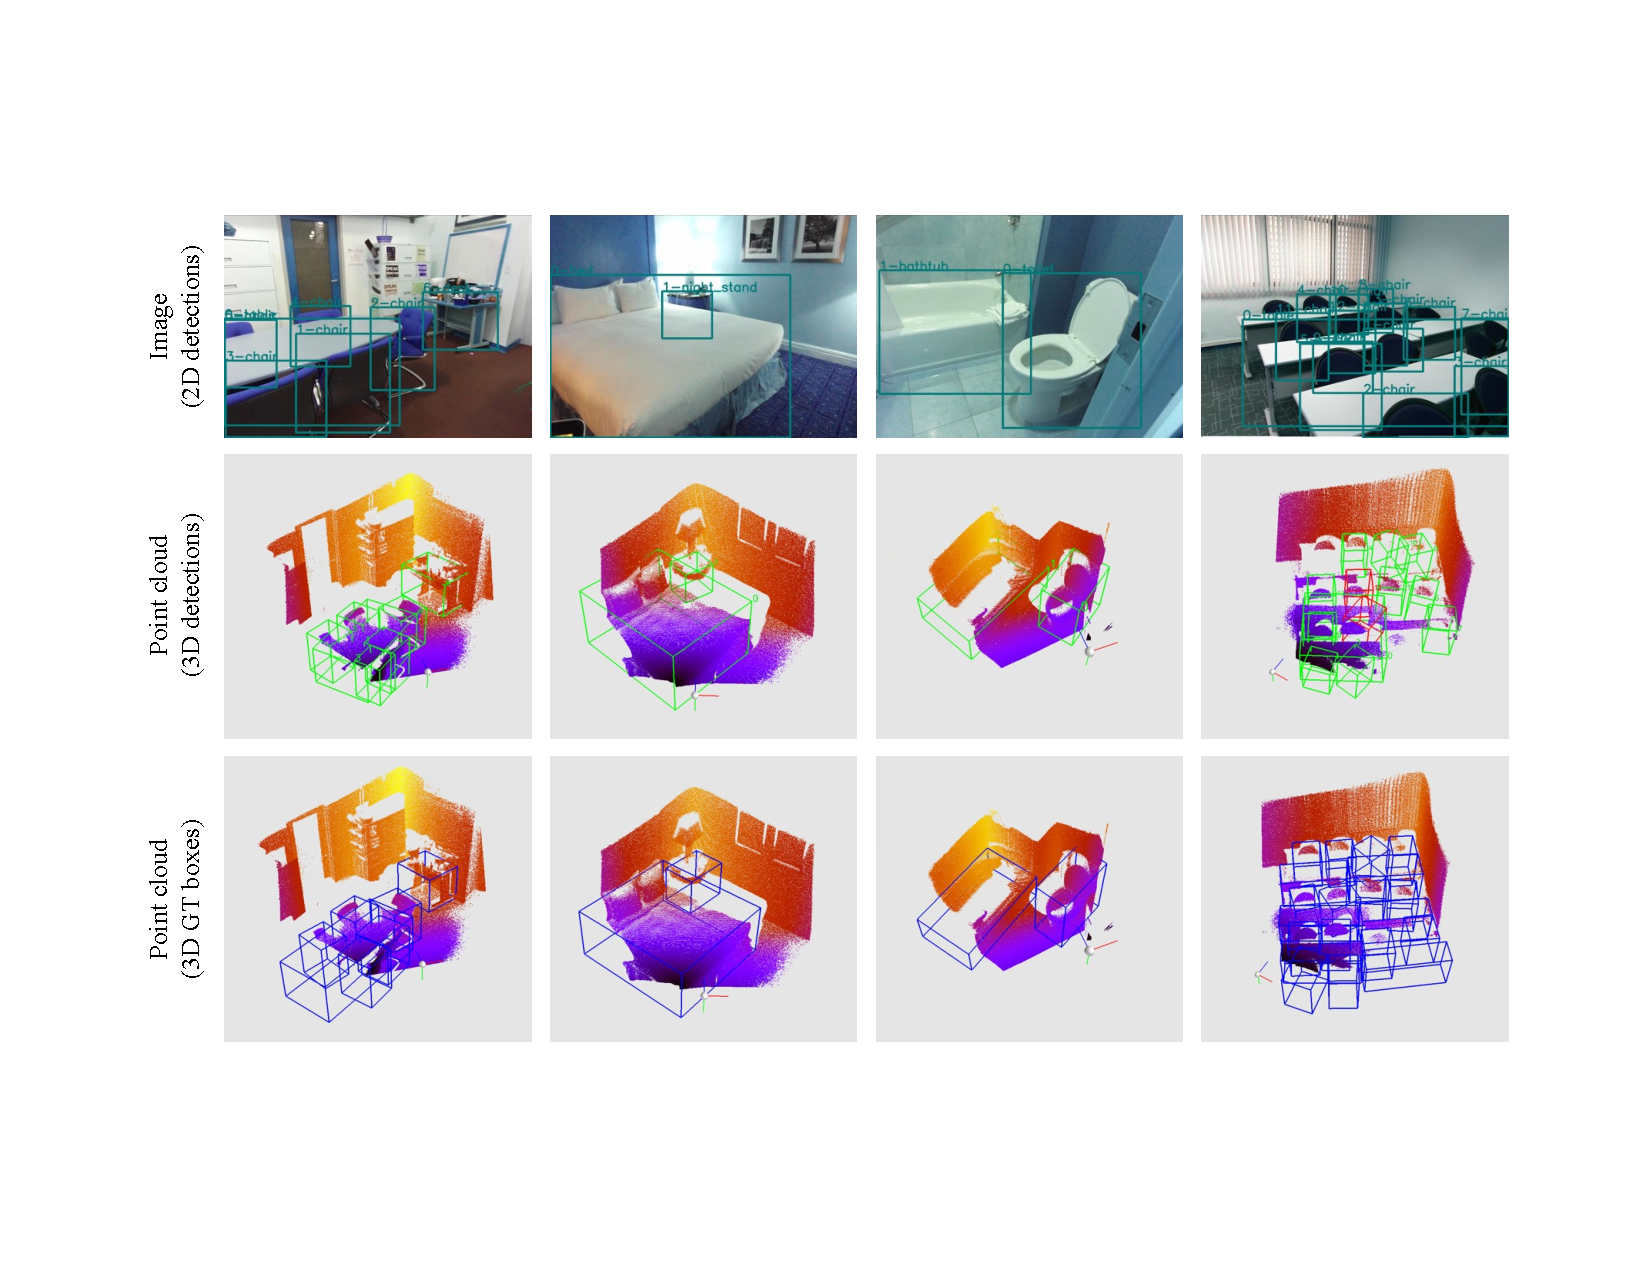
\includegraphics[width=0.95\linewidth]{./fig/sunrgbd_viz}
    \caption{\textbf{Visualization of Frustum PointNets results on SUN-RGBD val set.} \emph{First row:} RGB image with 2D detection boxes. \emph{Second row:} point cloud popped up from depth map and predicted amodal 3D bounding boxes (the numbers beside boxes correspond to 2D boxes on images). Green boxes are true positive. Red boxes are false positives. False negatives are not visualized. \emph{Third row:} point cloud popped up from depth map and ground truth amodal 3D bounding boxes.}
    \label{fig:sunrgbd_viz}
\end{figure*}

% \begin{table*}[]
%     \centering
%     \begin{tabular}{c|cccccccccc|c}
%     \hline
%     Category & bathtub & bed & bookshelf & chair & desk & dresser & nightstand & sofa & table & toilet & mAP \\ \hline
%          AP  & 81.26 & 56.73 & 67.17 & 64.14 & 77.83 & 33.29 & 37.22 & 57.41 & 49.92 & 43.53\\
%     Recall & 97.97 & 92.88 & 97.03 & 80.21 & 96.03 & 84.70 & 92.13 & 94.09 & 89.63 & 96.15 \\ \hline
%     \end{tabular}
%     \caption{\textbf{2D average precision (AP) and recall on SUN-RGBD val set.} IoU threshold is 0.5.}
%     \label{tab:my_label}
% \end{table*}

\begin{table*}[]
    \centering
    \begin{tabular}{l|cccccccccc|c}
    \hline
    Category & bathtub & bed & bookshelf & chair & desk & dresser & nightstand & sofa & table & toilet & mean \\ \hline
         AP (2D) & 81.3 & 56.7 & 67.2 & 64.1 & 77.8 & 33.3 & 37.2 & 57.4 & 49.9 & 43.5 & 50.3 \\ \hline
         AP (3D) & 43.3 & 81.1 & 33.3 & 64.2 & 24.7 & 32.0 & 58.1 & 61.1 & 51.1 & 90.9 & 54.0 \\ \hline
    \end{tabular}
    \caption{\textbf{2D and 3D object detection} AP on SUN-RGBD val set. 2D IoU threshold is 0.5. Note that on some categories we get higher 3D AP (displayed in the table as well, the same results as in main paper) than 2D AP because our network is able to recover 3D geometry from very partial scan and is also due to a more loose 3D IoU threshold (0.25) in SUN-RGBD 3D AP evaluation.}
    \label{tab:my_label}
\end{table*}


\begin{figure*}[t!]
    \centering
    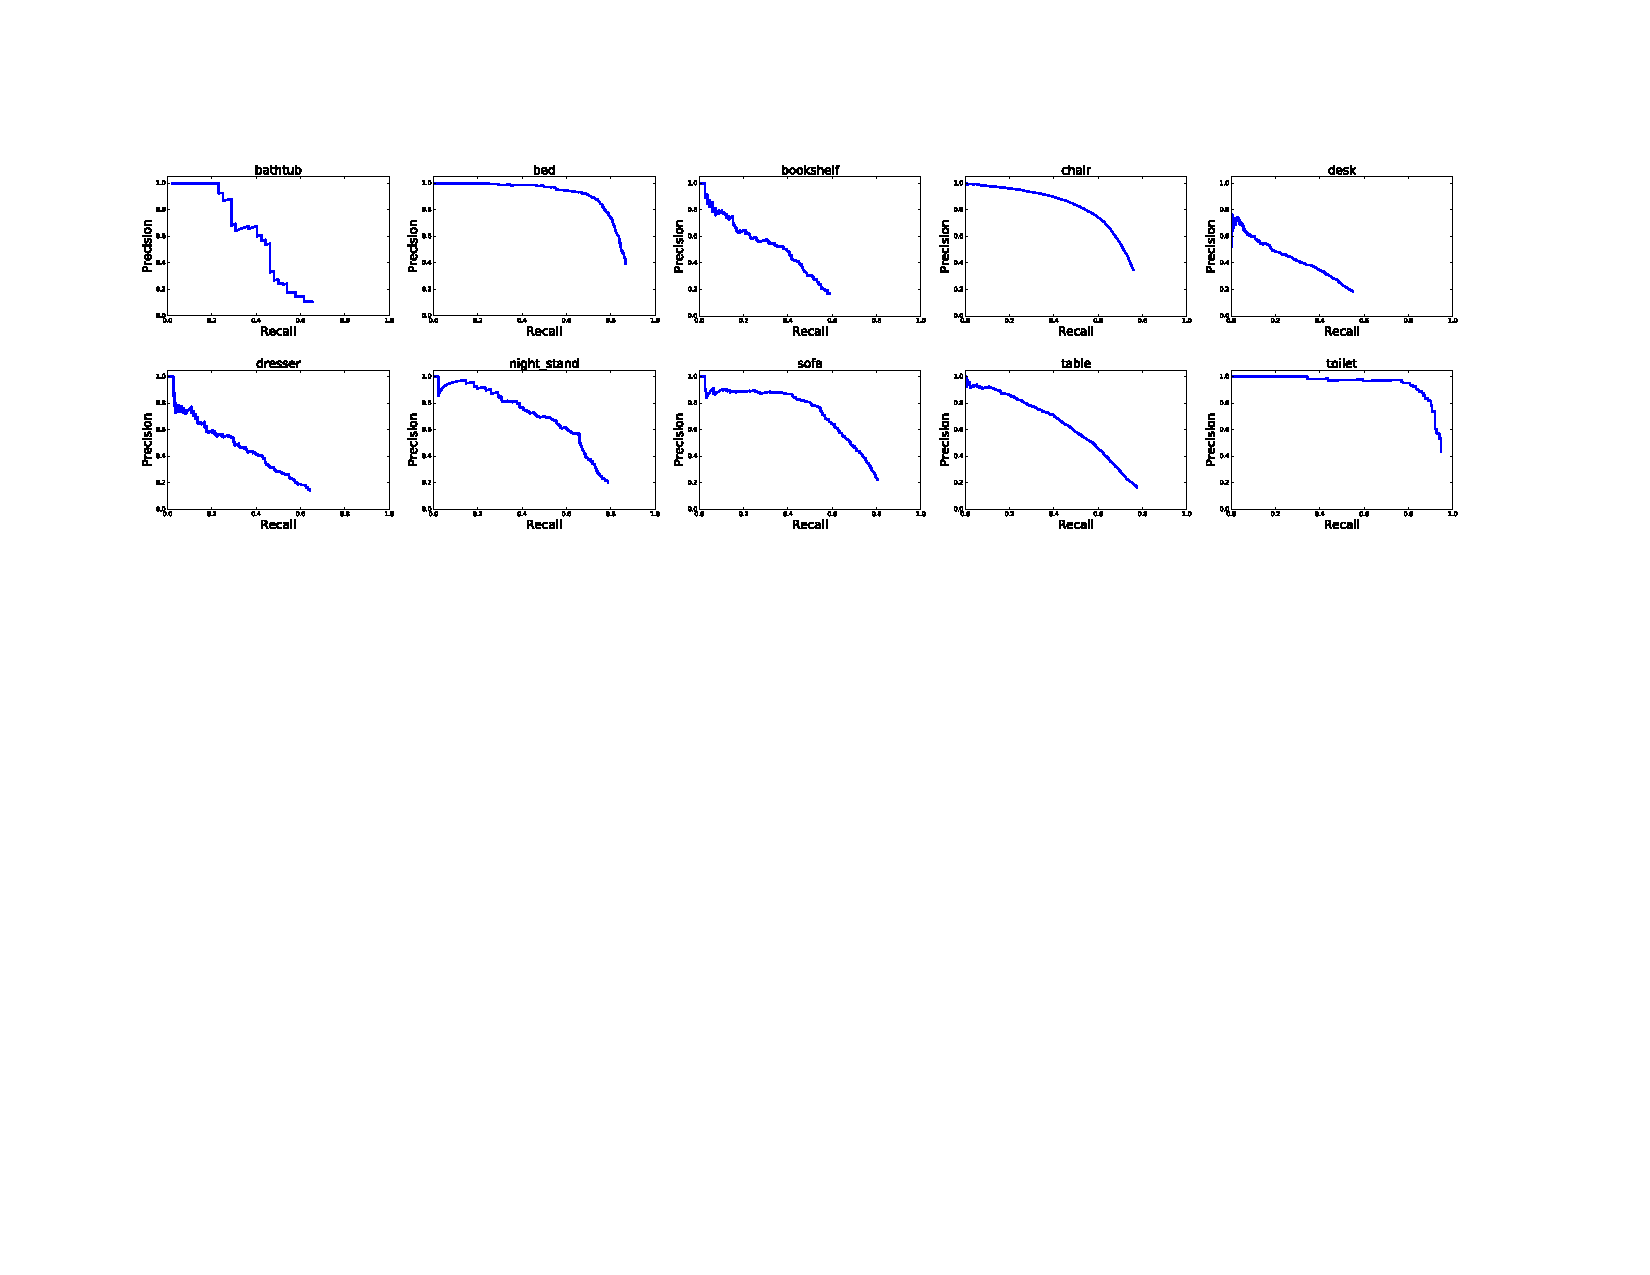
\includegraphics[width=\linewidth]{./fig/sunrgbd_3dap}
    \caption{\textbf{Precision recall (PR) curves} for 3D object detection on SUN-RGBD val set.}
    \label{fig:sunrgbd_ap}
\end{figure*}


